% !TEX TS-program = lualatex
% !TEX encoding = UTF-8 Unicode

% This is a simple template for a LaTeX document using the "article" class.
% See "book", "report", "letter" for other types of document.

\documentclass[12pt]{report} % use larger type; default would be 10pt

\usepackage[utf8]{inputenc} % set input encoding (not needed with XeLaTeX)
\usepackage{fontspec}
\setmainfont{Georgia}
\setsansfont{Georgia}
\setmonofont{Georgia}
%\usepackage[none]{hyphenat}
\usepackage{hyphenat}

%%% Examples of Article customizations
% These packages are optional, depending whether you want the features they provide.
% See the LaTeX Companion or other references for full information.

%%% PAGE DIMENSIONS
\usepackage{geometry} % to change the page dimensions
\geometry{a4paper, left=25mm, right=25mm, textwidth=85mm,columnsep=5mm, top=25mm}
\setlength{\parindent}{0pt}
% or letterpaper (US) or a5paper or....
% \geometry{margin=2in} % for example, change the margins to 2 inches all round
% \geometry{landscape} % set up the page for landscape
%   read geometry.pdf for detailed page layout information

\usepackage{subcaption}
\usepackage{graphicx} % support the \includegraphics command and options

\usepackage[parfill]{parskip} % Activate to begin paragraphs with an empty line rather than an indent

%%% PACKAGES
\usepackage{booktabs} % for much better looking tables
\usepackage{array} % for better arrays (eg matrices) in maths
\usepackage{paralist} % very flexible & customisable lists (eg. enumerate/itemize, etc.)
\usepackage{verbatim} % adds environment for commenting out blocks of text & for better verbatim
%\usepackage{subfig} % make it possible to include more than one captioned figure/table in a single float
\usepackage{amsmath}
% These packages are all incorporated in the memoir class to one degree or another...
\usepackage{lipsum}
%\usepackage{caption}
\usepackage{listings}

%%% HEADERS & FOOTERS
\usepackage{fancyhdr} % This should be set AFTER setting up the page geometry
\pagestyle{fancy} % options: empty , plain , fancy
\renewcommand{\headrulewidth}{0pt} % customise the layout...
\lhead{}\chead{}\rhead{}
\lfoot{}\cfoot{\thepage}\rfoot{}

%%% SECTION TITLE APPEARANCE
%\usepackage{sectsty}
%\allsectionsfont{\sffamily\mdseries\upshape} % (See the fntguide.pdf for font help)
% (This matches ConTeXt defaults)

%%% ToC (table of contents) APPEARANCE
\usepackage[nottoc,notlof,notlot]{tocbibind} % Put the bibliography in the ToC
\usepackage[titles,subfigure]{tocloft} % Alter the style of the Table of Contents
\renewcommand{\cftsecfont}{\rmfamily\mdseries\upshape}
\renewcommand{\cftsecpagefont}{\rmfamily\mdseries\upshape} % No bold!
\usepackage{authblk}

\usepackage{float}

\newcommand{\overbar}[1]{\mkern 1.5mu\overline{\mkern-1.5mu#1\mkern-1.5mu}\mkern 1.5mu}

%%% END Article customizations

%%% The "real" document content comes below...

\title{\textbf{Tunable electronic bands in twisted bilayer NbSe$_2$}}
\author{Conan Birkett}
\affil{Department of Physics, University of Bath, Bath BA2 7AY, United Kingdom}
%\date{} % Activate to display a given date or no date (if empty),
         % otherwise the current date is printed 

\begin{document}
\maketitle
\begin{abstract}
  Following observation of unconventional superconductive effects in twisted bilayer graphene, the novel field of 'twistronics' has seen a rapid progression in theory and experimentation. When a van der Waals heterostructure formed from a bilayer of 2D lattices is twisted at a so-called 'magic-angle', perturbation effects and interlayer tunneling lead to the formation of a flat electronic band at the Fermi level in some materials. These exotic electronic properties mean that these materials have the potential to be exploited as high temperature superconductors or in novel electronic devices. Using a multiorbital tight binding model (TBM), we model a bilayer of transition metal dichalcogenide 2H-NbSe$_2$ with interlayer tunneling at various twist angles. We observe splitting of electronic bands at degenerate eigenvalues, leading to nearly flat electronic bands near Fermi level for some twist angles. Our results show potential for further modelling of twisted bilayer NbSe$_2$ to affirm these promising properties.
\end{abstract}

\newpage

\section*{Introduction}

  In 2018, Cao Y. \textit{et al} \cite{Cao2018} realised unconventional superconductivity in bilayer graphene twisted to the 'magic-angle' of 1.1$^\circ$. This catapulted interest and research into graphene and two-dimensional (2D) materials to new heights. The potential of graphene in realising new electronic properties and phases of matter has been extensively explored both theoretically and experimentally.

  In recent years, focus has been directed at electrical properties of other 2D materials, like transition metal dichalcogenides (TMDCs), and into how combining multiple layers of 2D materials into van der Waals heterostructures can drastically effect their electronic properties. In particular, a novel field, dubbed 'twistronics' has grown from research into how relative interlayer twist in a van der Waals heterostructure influences the electronic properties of an electronic device. We examine such a heterostructure constructed from a bilayer of 2-hexagonal niobium diselenide (2H-NbSe$_2$); its monolayer is known to have different electronic properties from a bulk substrate: in particular a strong Ising-type spin-orbit coupling (SOC) that locks electron spins into out-of-plane directions.

  We show that perturbations introduced by the modelling of interlayer coupling cause electronic bands to seperate and avoid crossing at degenerate values \cite{Verhoeven1996, Cohen-Tannoudji2006}. We examine the effects of the perturbations by taking projections of low energy electronic bands onto unperturbed states (those without interlayer coupling). Further, there are points of interest particularily at saddle points between the $\Gamma$ and K critical points and near the M critical point, which display nearly flat electronic bands near the Fermi level at relatively large twist angles, much like bilayer graphene. These flat electronic bands are a result of the aforementioned band seperation. The high density of states associated with flat electronic bands at Fermi level is well studied in the context of novel electronic properties in other materials \cite{}, in particular magic-angle superconductivity in graphene \cite{}.

  Experimentally, it is possible to shift the Fermi level in a 2D system by a few hundred MeV by 'sandwiching' it within a capacitor \cite{}. Additionally, the large twist angle (compared to magic-angle graphene) at which these effects are observed could be more convenient for experimental realisation. Our results thus suggest tunable novel electronic properties and potentially flat electronic bands in bilayer $NbSe_2$ that are within experimental reach. However, further work is required in modelling the bilayer, as our model makes use of many non-trivial approximations. Significant improvements to the modelling of inter-layer tunneling must be made, and may have a drastic effect on the results presented. With this in consideration, our results are promising and justify further research into twisted bilayer $NbSe_2$.

  two states cross - interact and split - the stronger the coupling the further the split

 compare same twist angle with higher coupling - can see  bands seperate apart the levels are not degenerate but close - coupling makes them push apart by perturbation

 compare rotation at same strength 

 at saddle point, interesting things do not happen only at small twist angles

  could plot surfaces - where do they cross? at 15 degrees is it closer to saddle points?

if you can induce flatness (eg at 15 degrees some areas look flatter) in the electronic bands - leads to a high density of states (singularity - formally mathematically it tends to infinity) lots of electrons at this energy

flatness due to twist angles -> high density of states -> possible interesting effects

tunable! can change the properties of the material other than its metallic state normally - novel behaviour in the material is a good conclusion

figure font shouldnt be smaller than normal text - should probably be larger

\section*{Method}
  Our work draws on several published methods on NbSe2 and twistronics. In particular we draw upon the multiorbital tight binding model of monolayer NbSe2 from Habara and Wakabayashi\cite{Habara2021}. To model the bilayer with twist, we employ the method used in the original magic-angle paper by Bistritzer and MacDonald \cite{Bistritzer2011}. 

\subsection*{Monolayer NbSe2}
  NbSe$_2$ is a two-dimensional (2D) transition metal dichalcogenide (TMDC). Specifically, it belongs to the group V TMDCs with formula $MX_2$ for $M =$ Nb, Ta and $X =$ S, Se. It has metallic properties with superconductivity at temperatures below 7.2 K \cite{}. It also exhibits a strong spin-orbit coupling (SOC) field, which results in Ising-type SOC, i.e. a strong effective Zeeman field, which holds electron spins in out-of-plane directions.

  We employ a multiorbital tight binding model (TBM) of NbSe2, as described by Habara and Wakabayashi \cite{Habara2021}. We take a basis of $d_{z^2}$, $d_{x^2 - y^2}$ and $d_{xy}$ orbitals of the Nb atoms with SOC. These states are dominant in the electronic band near Fermi level. This basis is suitable for modelling the behaviour of low-energy electronic states in a NbSe$_2$ monolayer \cite{}.

\begin{figure}[t]
\centering
  \begin{subfigure}[c]{0.475\textwidth}
    \centering
    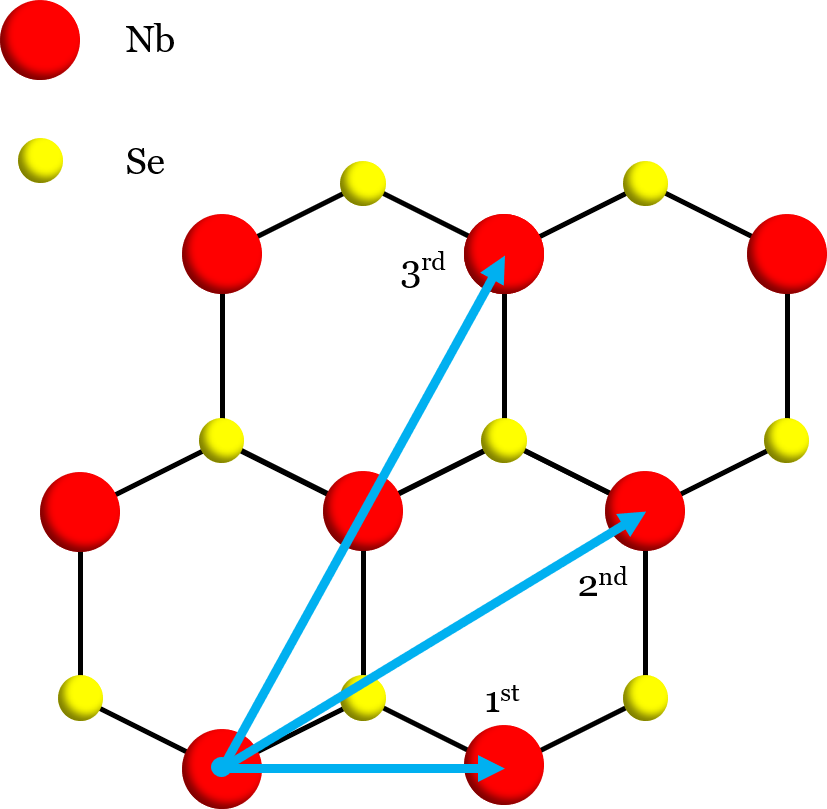
\includegraphics[width=0.95\textwidth]{NbSe_top.png}
    \caption{
      Top view of NbSe$_2$ with example nearest neighbours (NN) up to third NN sites.
    }
  \end{subfigure}
  \hfill
  \begin{subfigure}[c]{0.475\textwidth}
    \centering
    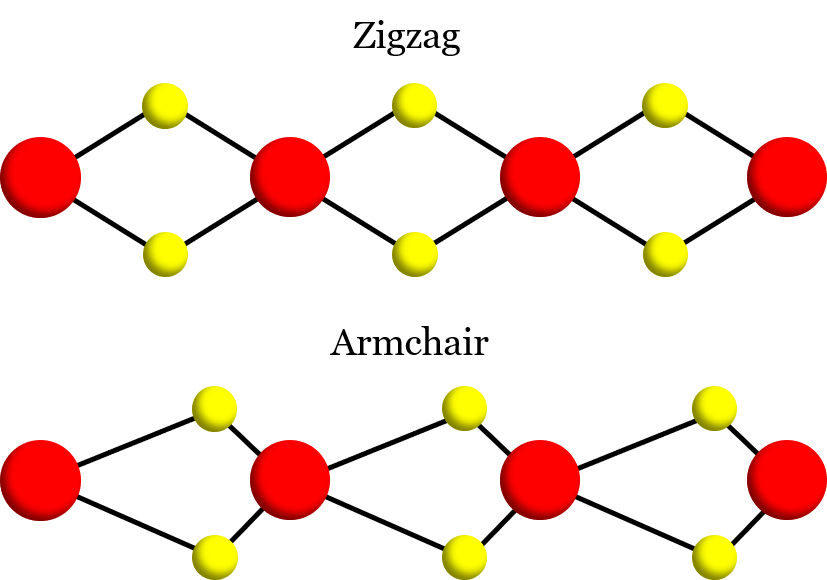
\includegraphics[width=0.95\textwidth]{NbSe_side.png}
    \begin{minipage}{.1cm}
      \vfill
    \end{minipage}
    \caption{
      Side view of NbSe$_2$ from the 'zigzag' and 'armchair' edges, Se atoms are directly above and below each other in out-of-plane axis.
    }
  \end{subfigure}
  \caption{
    Monolayer NbSe$_2$
  }
\end{figure}

\begin{figure}[t!]
\centering
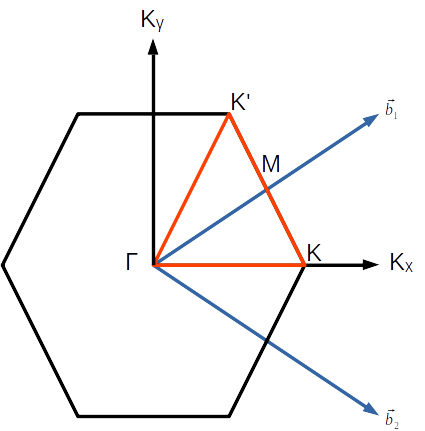
\includegraphics[width=0.6\columnwidth]{1st_BZ.png}
  \caption{
    First Brilloin zone in a hexagonal lattice. shown are: reciprocal lattice vectors $b_1, b_2$, standard critical points $\Gamma, K, K', M$ and wavevector axes $k_x, k_y$. Electronic bands are found for $k$ sampled from the equilateral triangle $\Gamma \rightarrow K \rightarrow M \rightarrow K' \rightarrow \Gamma$ or $\Gamma \rightarrow \Gamma$ shown in red.
  }
  \label{1st_BZ_diagram}
\end{figure}

  The TBM considers the interactions of these electronic states up to the third nearest neighbour sites.

  The eigenvalue equation of the TBM is 
      \begin{equation}
        \label{TBM_evalue_eqn}
        \hat{H}(k)\left|u_{n k}\right\rangle=E_{n k}\left|u_{n k}\right\rangle,
      \end{equation}

   where $k=\left(k_{x}, k_{y}\right)$ is the wave-number vector, $E_{nk}$ is the eigenvalue and $n = 1,2,\cdots,6$ is the band index.

   we define the eigenvector as
      \begin{equation}
        \begin{aligned}
          |u_{n k}\rangle=( & c_{n k, d_{z^{2}}, \uparrow}, c_{n k, d_{x y}, \uparrow}, c_{n k, d_{x^{2}-y^{2}}, \uparrow},\\
          & c_{n k, d_{z^{2}}, \downarrow}, c_{n k, d_{x y}, \downarrow}, c_{n k, d_{x^{2}-y^{2}}, \downarrow})^{T}
        \end{aligned}
      \end{equation}

  where $(\cdots)^T$ indicates the transpose of the vector and $c_{nk\tau s}$ is the amplitude at atomic orbital $\tau$ with spin $s$ for the $n$th energy band at $k$.

  The monolayer Hamiltonian $\hat{H}(k)$ with spin orbit coupling is then 
      \begin{equation}
        \hat{H}(k)=\hat{\sigma}_{0} \otimes \hat{H}_{\mathrm{TNN}}(k)+\hat{\sigma}_{z} \otimes \frac{1}{2} \lambda_{\mathrm{SOC}} \hat{L}_{z}
        \label{monolayer_hamitonian}
      \end{equation}

  with the TBM nearest neighbour Hamiltonian

      \begin{equation}
        \hat{H}_{\mathrm{TNN}}(k)=\left(\begin{array}{ccc}
        V_{0} & V_{1} & V_{2} \\
        V_{1}^{*} & V_{11} & V_{12} \\
        V_{2}^{*} & V_{12}^{*} & V_{22}
        \end{array}\right)
      \end{equation}

  and spin orbit coupling term

      \begin{equation}
        \hat{L}_{z}=\left(\begin{array}{ccc}
        0 & 0 & 0 \\
        0 & 0 & -2 i \\
        0 & 2 i & 0
        \end{array}\right)
      \end{equation}

  $\hat{\sigma}_0$ and $\hat{\sigma}_z$ are Pauli matrices and $\lambda_{\text{SOC}}=0.0784$ eV is the Ising-type SOC parameter. The potentials $V_0 \cdots V_{22}$ in the TNN Hamiltonian are functions of $k$ determined from the nearest neighbour hopping vectors with fitting parameters.

  The resulting monolayer Hamiltonian $\hat{H}(k)$ is a 6x6 block diagonal Hermetian matrix as a function of wavevector $k$. The eigenvalues of this Hamiltonian correspond to the energy of the 6 eigenstates / electronic bands for a given point in reciprocal space $k$. When determining the electronic bands, we take $k$ from slices in the first Brillouin zone along the standard critical points: $\Gamma, K, K', M$. Using Bloch's theorem we can describe the electronic properties of the whole monolayer by considering the region bounded by these points due to the periodicity of potentials in the lattice and reflectional symmetry. Specifically, $k$ bounded by the equilateral triangle $\Gamma \rightarrow K \rightarrow M \rightarrow K' \rightarrow \Gamma$, hereafter refered to as $\Gamma \rightarrow \Gamma$.

\subsection*{Modelling a twist}

  Before constructing a twisted bilayer, we first consider a monolayer twisted by some angle $theta$. A rotation in primitive lattice vectors $a_1, a_2 \rightarrow a_1', a_2'$ corresponds to the same rotation in reciprocal lattice vectors $b_1, b_2 \rightarrow b_1', b_2'$. We can treat this rotation as a rotation of the coordinate system in $k$ space: $(k_x, k_y) \rightarrow (k_x', k_y')$. Then, for some vector $k' \in (k_x', k_y')$, we can find the same vector $k'$ in our original wavevector basis $(k_x, k_y)$ by rotating it by $-\theta$.

\begin{figure*}[t]
\centering
  \begin{subfigure}[t]{0.475\textwidth}
    \centering
    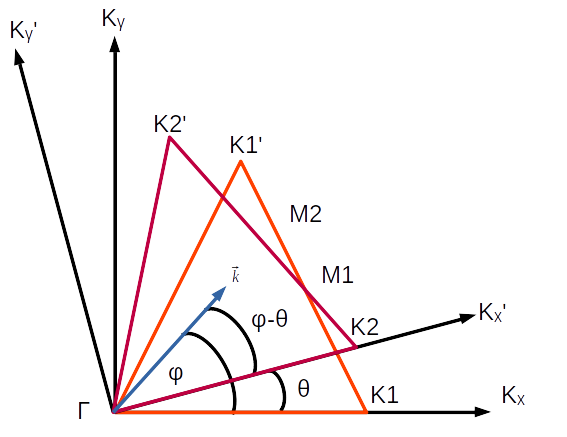
\includegraphics[width=0.95\textwidth]{twisted_triangles.png}
    \caption{
      Equilateral triangle from first Brillouin zone shown in unrotated and relatively rotated (by angle $\theta$) reciprocal coordinate systems. An arbitrary vector $k$ in the rotated basis $(k_x', k_y')$ must first be rotated by $-\theta$ before it can be projected onto the unrotated basis $(k_x, k_y)$
    }
    \label{twisted_triangles}
  \end{subfigure}
  \hfill
  \begin{subfigure}[t]{0.475\textwidth}
    \centering
    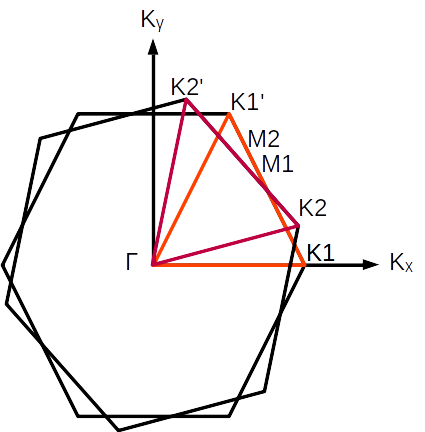
\includegraphics[width=0.95\textwidth]{heterostructure_BZ_path.png}
    \caption{
      Brillouin zones of both layers at relative angle $\theta$ overlayed. Evaluation of the electronic bands is taken on the set $\Gamma \rightarrow K1 \rightarrow M1 \rightarrow K1' \rightarrow \Gamma \rightarrow K2 \rightarrow M2 \rightarrow K2' \rightarrow \Gamma$ or $\Gamma \rightarrow \Gamma \rightarrow \Gamma$.
    }
    \label{heterostructure_BZ_path}
  \end{subfigure}
  \caption{
  }
\end{figure*}

  If we consider the equilateral triangle in reciprocal space $\Gamma \rightarrow K1 \rightarrow M1 \rightarrow K1' \rightarrow \Gamma$ taken on an unrotated basis, we can construct a rotated triangle $\Gamma \rightarrow K2 \rightarrow M2 \rightarrow K2' \rightarrow \Gamma$. For the evaluation of electronic bands in a twisted bilayer we sample $k$ from the path $\Gamma \rightarrow K1 \rightarrow M1 \rightarrow K1' \rightarrow \Gamma \rightarrow K2 \rightarrow M2 \rightarrow K2' \rightarrow \Gamma$, or in shorthand $\Gamma \rightarrow \Gamma \rightarrow \Gamma$

\subsection*{Twisted bilayer}

  NbSe$_2$ monolayers are held together by a weak van der Waals interaction. This allows for the stacking of multiple layers - specifically a bilayer. Because of the relatively weak bonding between layers it is possible to orient these layers at twist angles relative to each other. Through this rotation and by inter-layer tunneling, we aim to explore novel electronic properties in twisted bilayers.

  To describe the electronic states in a twisted bilayer we can initially start with a simple model with no interaction between states in different layers. We construct the Hamiltonian of the whole system by taking a block diagonal Hamiltonian matrix $\hat{H}{k}$ from two monolayer matrices $\hat{H_1}{k}$ and $\hat{H_2}{k'}$
%
      \begin{equation}
        \hat{H}(\boldsymbol{k})=\left(\begin{array}{cc}
          \hat{H_1}(\boldsymbol{k}) & 0\\
          0 & \hat{H_2}(\boldsymbol{k'})
        \end{array}\right)
        \label{simple_bilayer_hamiltonian}
      \end{equation}
      
  where $\hat{H_2}(k')$ is the Hamiltonian of the second monolayer, which is rotated by angle $\theta$ relative to the first. To find $\hat{H}(k)$ we must rotate $k$ to $k'$ (as described previously) in $\hat{H_2}(k')$.

  Continuing, we will denote rotated vectors as $v'$, where the rotation is relative to a vector on the 'unrotated layer', $v$. We will also denote these layers by index, layer 1 is unrotated, layer 2 is rotated relative to layer 1.

\subsection*{Interlayer tunneling}
  To model inter-layer electron tunneling, we follow the method of Bistritzer and MacDonald \cite{Bistritzer2011} for graphene, which is outlined for a more general case by Koshino \cite{Koshino2015}.

  For reciprocal lattice vectors $b_i, b_i'$ where $b_i'$ is the equivalent reciprocal lattice vector of the rotated layer, we can show that
  \begin{equation}
    k + G = k' + G',
    \label{inter-layer_k_plus_G}
  \end{equation}
  where $G = m_1 b_1 + m_2 b_2 \text{ and } G' = m_1 b_1' + m_2 b_2'$ are reciprocal lattice vectors of the unrotated and rotated layers respectively.

  This is because a Bloch state on layer 1 $\phi_k^{(1)}$ is a summation of $e^{i(k+b)}$ over reciprocal vectors. Similarily, on layer two $\phi_{k'}^{(2)}$ is a sum over $e^{i(k'+b')}$. The system Hamiltonian is described by Fourier components of $G, G'$. So the matrix element $\langle \phi_{k'}^{(2)} | \hat{H} | \phi_{k}^{(1)}$ is only non-zero if \ref{k_plus_b} holds. The derivation of \ref{k_plus_b} is as follows:

  First we assume that equivalent unit cells in both layers $X$ and $X'$ have multiple atomic orbitals with real space lattice positions
  \begin{equation}
    \begin{gathered}
    R_X = n_1 a_1 + n_2 a_2 + \tau_X,\\
    R_{X'} = n_1 a_1' + n_2 a_2' + \tau_{X'},
    \end{gathered}
    \label{inter-layer_real_sublattice_positions}
  \end{equation}

  for $n_1, n_2 \in \mathrm{N}$ and primitive lattice vectors $a_1, a_2$ and $a_1', a_2'$ in either layer respectively. $\tau_X$ are the sublattice positions of the atomic states in unit cell $X$.

  We define $| R_x \rangle \equiv \phi(r - R_X)$ as the atomic state of sublattice $X$ at localised real position $R_X$.

  The interlayer Hamiltonian elements are then
  \begin{equation}
    U = -\sum_{X, X'} T_{X'X}(R_{x'} - R_x) |R_{x'}\rangle \langle R_x|,
    \label{inter-layer_hamiltonian_elements}
  \end{equation}

  where the inter-layer transfer potential $-T_{X'X}(R_{x'} - R_x)$ is a function of the real space positions of the atomic orbitals, the specifics of this function we shall discuss later.

  We define the Bloch basis in each layer as the summation over unit cells (and thus primitive lattice vectors)
  \begin{equation}
    | k,j,l \rangle = \frac{1}{\sqrt{N_l}}\sum_{R_X}e^{ik\cdot(R+\tau_i)}\phi_j(r-R-\tau_j, z-z_l)
    \label{inter-layer_real_bloch_basis}
  \end{equation}

  for wavevector $k$, sublattice $j$ and layer index $l$ where $N_l$ is the number of unit cells in layer $l$. $\phi_j (r - R - \tau_j, z-z_l)$ is the wavefunction in 2D real space in the plane and out of plane.

  Our inter-layer hopping Hamiltonian elements are then given by
  \begin{multline}
    \langle k',j',l' | U | k, j, l \rangle = \\
    \frac{1}{\sqrt{N_l N_{l'}}} \sum_{R, R'} e^{ik \cdot (R+\tau_j)} e^{-ik' \cdot (R' + \tau_{j'})} \times \langle \phi_{j'}(r - R' - \tau_{j'}, z - z_{l'}) | U | \phi_j (r - R - \tau_j, z - z_l)\\
     =\frac{1}{\sqrt{N_l N_{l'}}} \sum_{R, R'} e^{ik \cdot (R+\tau_j)} e^{-ik' \cdot (R' + \tau_{j'})} \times t(R'-R +\tau_{j'} - \tau_j, z_l' - z_l),
    \label{}
  \end{multline}

  where we invoke a two centre approximation, the hopping between sites is a function of their distance only. We also assume that the the hopping $t(\vec{r_{2D}}, z)$ does not depend on the direction of $\vec{r_{2D}}$ i.e. $t(\vec{r_{2D}}, z) = t(|\vec{r_{2D}}|, z)$

  For a large superlattice period, the relative inter atomic positions for every combination of atomic sites are required. It is easier to reconstruct the Hamiltonian in reciprocal space.

  By taking a Fourier transform (see appendix) we can show that
  \begin{equation}
    \langle k',j',l' | U | k, j, l \rangle = \sum_{G, G'} t(k'+G', z) \delta_{k-G, k'+G'},
    \label{inter-layer_hopping_elements}
  \end{equation}
  
  which yields the result in \ref{inter-layer_k_plus_G}
  
  As we are taking the interlayer tunneling to be a function of $k+G$, we only consider $G, G'$ of magnitude $\leq$ the reciprocal lattice constant $b$. The result is that for a given $k, k'$ we have seven pairs of permissible $G, G'$ that obey \ref{inter-layer_k_plus_G} we define them as follows: $G_0$ is the zero vector; $G_1, G_2$ are equal to reciprocal lattice vectors $b_1, b_2$; $G_{3,\cdots,6}$ continue from reciprocal lattice vectors in a clockwise fashion in 60$^\circ$ intervals.

  We define
  \begin{equation}
    G_i^M = G_i - G_i'
    \label{inter-layer_G_M_def}
  \end{equation}
  such that \ref{inter-layer_k_plus_G} becomes
  \begin{equation}
    k' = k + G^M
    \label{inter-layer_k_plus_G_M}
  \end{equation}

  So for a given point on layer one $k_0$, we have a well defined set of permissible $k'$ points on the second layer between which tunneling is allowed.

\subsection*{Tunneling potential and Hamiltonian}

The tunneling potential $t(k + G, z)$ we model as a Gaussian in the in-plane axes and assume $z$ is constant
\begin{equation}
  t(k + G) = \frac{C\pi}{A_{UC} r_0^2}e^{- r_0^2 (k + G)/4}
\end{equation}

Due to time limitations, in our actual results we use a constant tunneling potential of 0.1eV. We then assume that the potential is negligible for large $k + G$ so we will only allow tunneling to the first, where $|G|$ is equal to the reciprocal lattice constant

Talk about the allowed tunneling between different k'!!! eg 

\begin{figure}[t!]
\centering
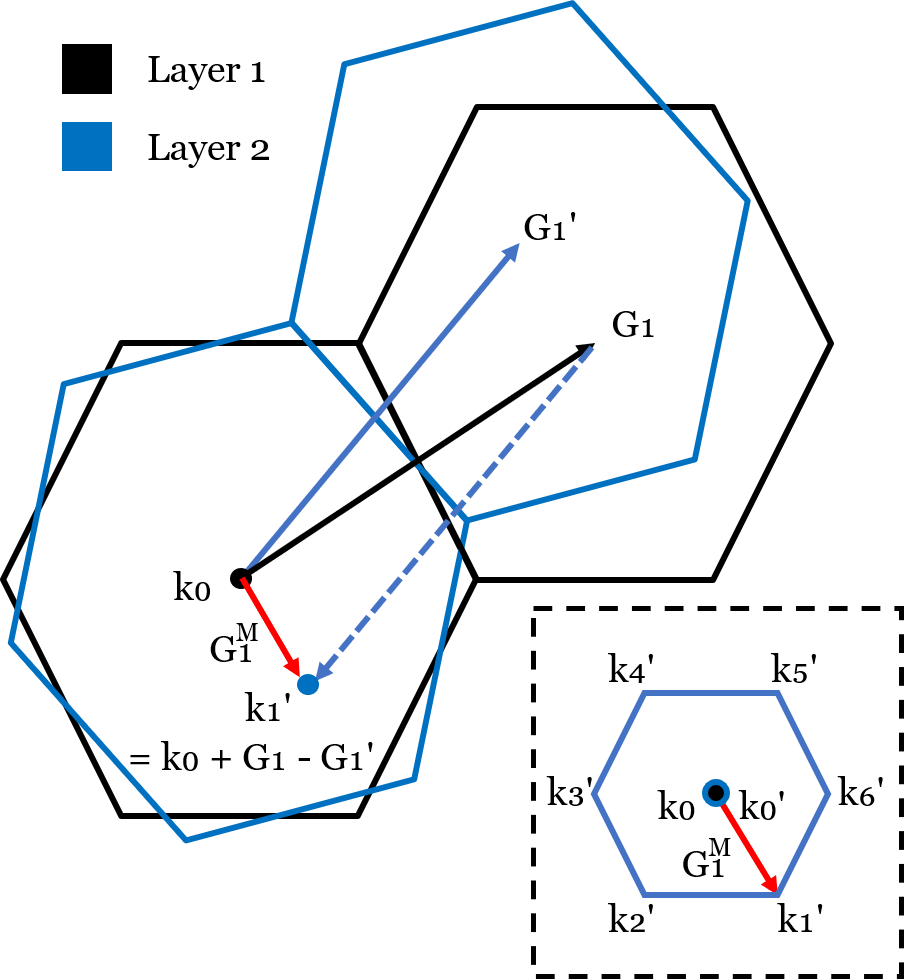
\includegraphics[width=0.6\columnwidth]{k_prime_diagram.png}
  \caption{
    The relationship described by \ref{inter-layer_k_plus_G_M} implies that for a point $k$ on one layer, there are seven points $k'$ on the other layer between which tunneling is allowed (shown in the insert box) }
  \label{inter-layer_k_prime_diagram}
\end{figure}

  Previously our Hamiltonian was a $12\times12$ function of $k$. Now, with the  addition of inter-layer tunneling we have an $84\times84$ Hamiltonian with interlayer tunneling potential on the off-diagonal blocks. We assume that the inter-layer tunneling is negligible for $d_xy$ and $d_{x^2-y^2}$ orbitals as they exist primarily in the in-plane axis, so when constructing the Hamiltonian we only allow tunneling between $d_{z^2}$ orbitals.

\subsection*{Avoided crossing in degenerate electronic bands}

\begin{figure}[t!]
\centering
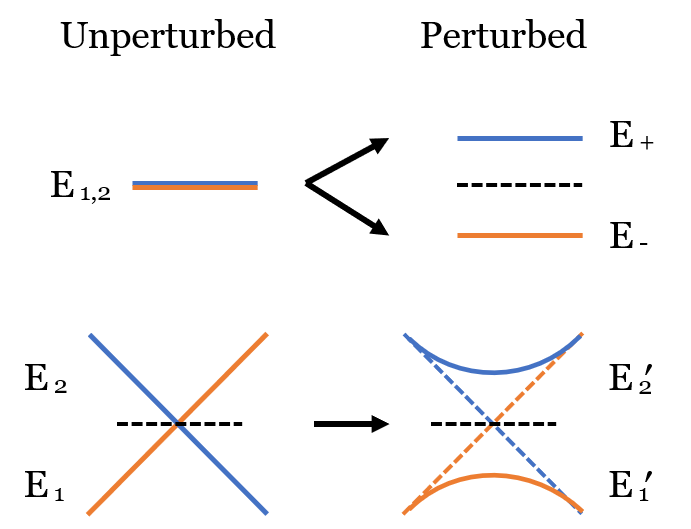
\includegraphics[width=0.6\columnwidth]{splitting_bands_diagram.png}
  \caption{Introducing a coupling perturbation to a Hamiltonian with degenerate eigenvalues results in the eigenvalues seperating. In electronic bands this manifests as the bands splitting into two hyperbola at points where they previously would've crossed (degeneracy).}
  \label{splitting_bands}
\end{figure}

A well studied phenomena in quantum mechanics is the splitting of degenerate electronic states under a perturbation \cite{Verhoeven1996, Cohen-Tannoudji2006}. This can be simply explained using an example two state model with Hamiltonian
%
\begin{equation}
  H = \begin{pmatrix}
        E_1 & 0 \\
        0 & E_2 \\
      \end{pmatrix}
      \text{ with eigenvectors }
      \begin{pmatrix}
        1\\
        0\\
      \end{pmatrix},
      \begin{pmatrix}
        0\\
        1\\
      \end{pmatrix},
\end{equation}
for some potentials $E_1$, $E_2$. If $E = E_1 = E_2$ then there is twofold degeneracy in the Hamiltonian. Introducing a simple permutation in the form of a potential coupling $W$ between the basis states
\begin{equation}
  H' = H + P =\begin{pmatrix}
    E_1 & 0 \\
    0 & E_2 \\
  \end{pmatrix}
  +\begin{pmatrix}
    0 & W \\
    W* & 0 \\
  \end{pmatrix}
  =\begin{pmatrix}
    E_1 & W \\
    W* & E_2 \\
  \end{pmatrix},
  \label{perturbation_matrix}
\end{equation}
upon diagonalising the modified Hamiltonian we find new eigenvalues 
\begin{equation}
\begin{gathered}
  E_{+, -} = {\frac{1}{2}(E_1 + E_2)} \pm {\frac{1}{2}\sqrt{(E_1-E_2)^2+4|W|^2}},\\
  \text{or, when } E = E_1 = E_2, \quad E_{+,-} = E \pm |W|.
\end{gathered}
  \label{perturbation_energy}
\end{equation}

The perturbation also alters the eigenvectors of the Hamiltonian, they exist as a linear combination of the original unperturbed eigenstates. This principle can be seen in the splitting of electronic (Bloch) bands with the introduction of a perturbation. In FIG \ref{splitting_bands} we show an example crossing point (degeneracy) of electronic bands and their modification due to perturbation, the result is that the crossing point becomes two hyperbola and the bands are no longer degenerate \cite{Cohen-Tannoudji2006, Verhoeven1996}. The strength of the band seperation is dependent on the difference between two similar energy levels $E_1 - E_2$, that is, this effect is most prevalent at degenerate and nearly degenerate eigenvalues - near crossing points. As the energy difference between bands increases the hyperbola asymtotically approach the non-degenerate case.

\subsection*{Implementation}
The implementation of these methods and graphing of their results was done in Python using the NumPy library

\section*{Results}

\subsection*{Monolayer electronic bands}
Initially, we seek to reproduce the tight binding bands from Habara et al \cite{Habara2021}. Using their matrix elements we reproduce the six electronic bands corresponding to the $d_{z^2}$, $d_{x^2 - y^2}$ and $d_{xy}$ orbitals of the Nb atoms with SOC. The result in FIG \ref{monolayer_bands} is a reproduction of the bands shown in FIG 1 d) of Habara \cite{Habara2021}. Whilst not a novel result, it is a useful benchmark for checking the validity of further results. Note that Habara et al sample the bands on a different path in $k$ space, in particular they sample on the path  $M \rightarrow K' \rightarrow \Gamma \rightarrow K \rightarrow M$. So whilst we show the same bands, the $k$ space axis is arranged differently. The NbSe$_2$ monolayer bands predict the electrical properties of the monolayer, in particular that it is metallic.

\begin{figure}[t!]
\centering
  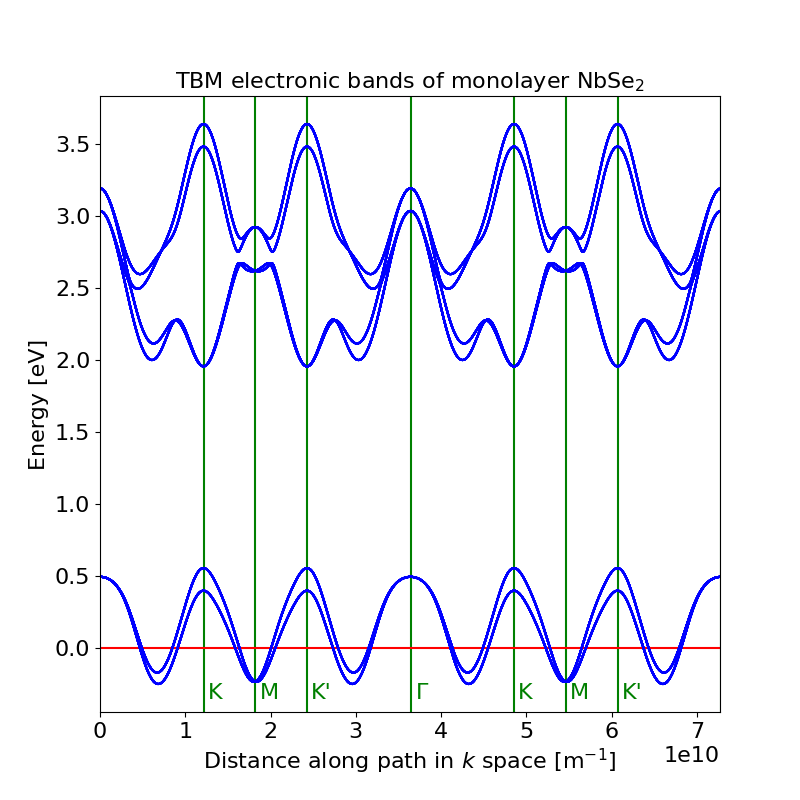
\includegraphics[width=0.6\columnwidth]{monolayer_bands.png}
  \caption{
    Reconstruction of FIG 1 d) from Habara et al \cite{Habara2021}. 6 Electronic bands are produced from the nearest neighbour tight binding model (TBM) that incorporates $d_{z^2}$, $d_{x^2 - y^2}$ and $d_{xy}$ orbitals of Nb atoms with spin orbit coupling. The conduction band on the Fermi level (shown in red) tells us that monolayer NbSe$_2$ is metallic. The relatively high spin orbit coupling in NbSe$_2$ produces the meV scale splitting of bands seen near the $K$ critical points.
  }
  \label{monolayer_bands}
\end{figure}

\subsection*{Bilayer electronic bands}
Following the monolayer bands, we construct a Hamiltonian of two layers, with one rotated at some twist angle $\theta$ as in eq \ref{simple_bilayer_hamiltonian}. The graphs in FIG \ref{bilayer_bands} show the electronic bands of both layers with $5^\circ$ and $15^\circ$ relative rotation. The bands are sampled from the constructed path $\Gamma \rightarrow \Gamma \rightarrow \Gamma$ in $k$ space seen in figure \ref{heterostructure_BZ_path}. The graphs in FIG \ref{bilayer_bands} show 12 electronic bands, with 6 from each layer. Because of the construction of the path in $k$ space, there are always 6 bands which appear exactly as in FIG \ref{monolayer_bands}. The remaining 6 bands are those sampled from one of the triangular paths that is rotated relative to the layer they exist on. This results in discontinuities in the bands as the corners of the triangular paths are discontinuous in the 2D $k$ space plane. The geometric reasoning for the apparent discontinuities is better seen in FIG \ref{surface_plot}, where the lowest energy band as seen in FIG \ref{bilayer_bands} is shown on the triangular path it takes, plotted above a surface plot of the whole 2D band in the same sampling region of the Brillouin zone. Again, nothing physically novel can be inferred from these graphs other than that the model up to this point is functional. They simply represent two sets of electronic states corresponding to two layers of NbSe$_2$, with no notion of interaction, coupling, or distance between layers - only a twist relative to each other. 

talk about rotation / unrotation

Because of the paths in $k$ space taken, these graphs are mirrored about the $\Gamma$ that seperates the first and second triangular paths.
%
\begin{figure*}[t!]
\centering
  \begin{subfigure}[t]{0.45\textwidth}
    \centering
    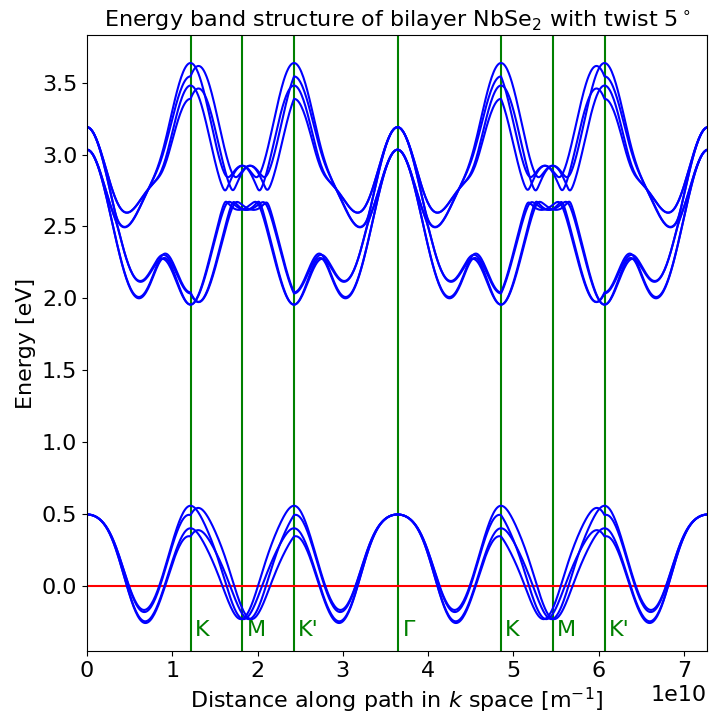
\includegraphics[width=0.95\textwidth]{bilayer_bands_5.png}
    \caption{
      Relative twist 5$^\circ$
    }
    \label{bilayer_bands_5}
  \end{subfigure}
  \hfill
  \begin{subfigure}[t]{0.45\textwidth}
    \centering
    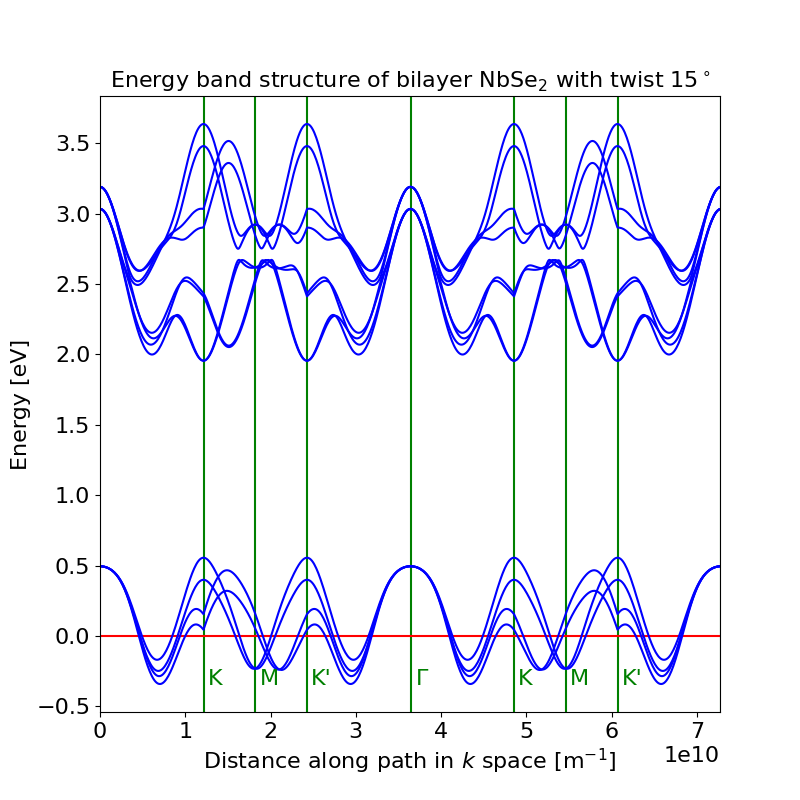
\includegraphics[width=0.95\textwidth]{bilayer_bands_15.png}
    \caption{
      Relative twist 15$^\circ$
    }
    \label{bilayer_bands_15}
  \end{subfigure}
  \caption{
    Bilayer band structure accounting for rotation with no inter-layer coupling. This graph is equivalent to FIG \ref{monolayer_bands} for two monolayers at once, one with a relative twist to the other. The bands are sampled from two triangular paths in $k$ space, one after the other. These paths join the critical points of symmetry the Brillouin zone in the unrotated and then rotated lattices as in FIG \ref{twisted_triangles}
  }
  \label{bilayer_bands}
\end{figure*}

\subsection*{Inter-layer tunneling}
With the model capable of describing a bilayer with relative twist, we now seek to introduce some inter-layer interaction in the form of coupling by electron tunneling. From the relationship in (\ref{inter-layer_k_plus_G_M}) we found that for each state at point $k$ on one layer, there are a set of $k'$ on the other layer between which tunneling is allowed. We further reduce this set of $k'$ points to seven points for practical computation. To model the tunneling between these points, we expand the Hamiltonian to describe 84 states - using a fixed tunneling coefficient $t(k + G) = \text{const}$ for the allowed interactions. The result is 84 eigenstates at each $k$, generating 84 electronic bands. In FIG \ref{bilayer_bands_coupled} we show the bands with energies near the Fermi level only. The perturbations introduced by the tunneling causes points where bands previously were crossed (degeneracy) to seperate into higher and lower energies as previously described in (\ref{perturbation_matrix}) and (\ref{perturbation_energy})

\begin{figure*}[t!]
\centering
  \begin{subfigure}[t]{0.45\textwidth}
    \centering
    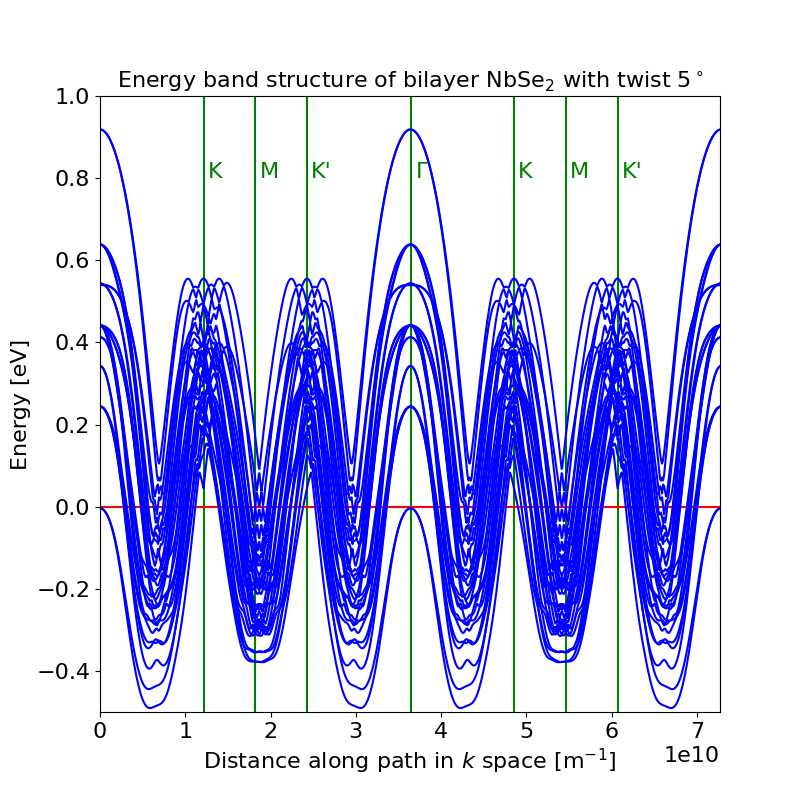
\includegraphics[width=0.95\textwidth]{bilayer_bands_5_coupled.png}
    \caption{
    }
    \label{bilayer_bands_5_coupled}
  \end{subfigure}
  \hfill
  \begin{subfigure}[t]{0.45\textwidth}
    \centering
    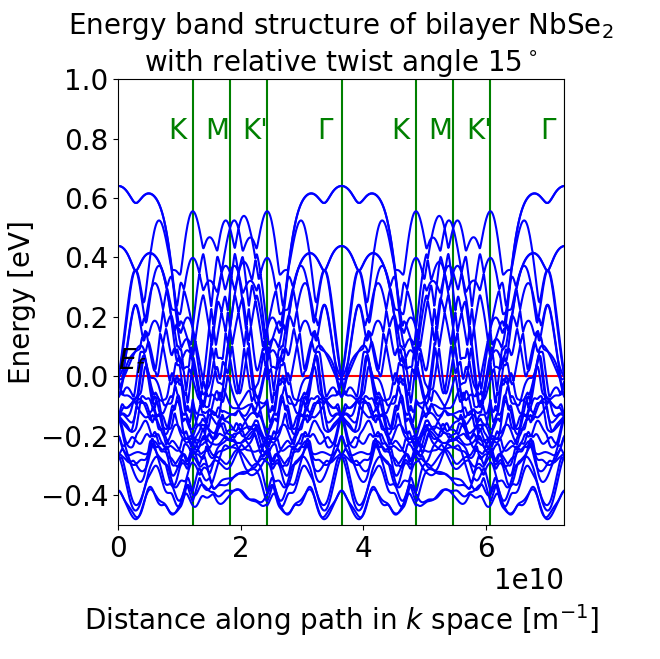
\includegraphics[width=0.95\textwidth]{bilayer_bands_15_coupled.png}
    \caption{
    }
    \label{bilayer_bands_15_coupled}
  \end{subfigure}
  \caption{Electronic bands near the Fermi level $E_f$ with interlayer coupling $t(k+G)$ potential set to 0.1 eV. A basis of 84 states is used to model the inter-layer tunneling, resulting in 84 electronic bands.}
  \label{bilayer_bands_coupled}
\end{figure*}

To better understand the effects of inter-layer tunneling we take a projection (inner product) of each of the 84 bands seen in FIG \ref{bilayer_bands_coupled} onto the lowest energy unperturbed states at $k_0 = k$ only - as seen in FIG \ref{bilayer_bands}. We then examine the effects of varying the fixed coupling potential and inter-layer twist angle in FIG \ref{bilayer_bands_projected_coupling} and FIG \ref{bilayer_bands_projected_rotation} respectively. In these graphs the opacity of the states (shown in red) is given by the numerical value of the projection.

Firstly we examine how altering the fixed coupling potential effects the band structure in FIG \ref{bilayer_bands_projected_coupling}, setting $t(k+G) = 0.05, 0.1, 0.2 \text{ and } 0.4$ eV and inter layer rotation to 15$^\circ$. There are two main observations: firstly, the interlayer coupling perturbation results in the splitting of the degenerate bands. This is best seen at the $\Gamma$ critical points where the two bands shown are almost indistinguishable. This degeneracy results in a large splitting of the bands as predicted by the simpler two state model in (\ref{perturbation_matrix, perturbation_energy}). As well as the low energy difference increasing the splitting of the bands, the strength of the coupling potential also increases the magnitude of the splitting.

The second observation is an increase in the perturbed electronic states formed from these two low energy unperturbed states at $k_0$.

CHECK THIS This makes sense as the full band structure contains hybrid states that exist partly on the other $k'$ points that tunneling is allowed between, so as the tunneling potential is increased, we see a greater dispersion of these states onto the two unperturbed states at $k_0$ shown.

\begin{figure*}[t]
\centering
  \begin{subfigure}[b]{0.475\textwidth}
    \centering
    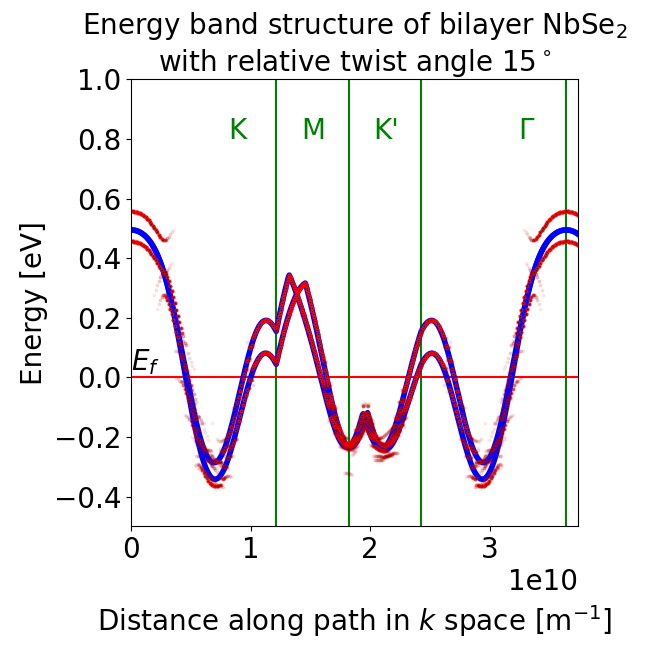
\includegraphics[width=0.95\textwidth]{0.05_coupling_15_deg.png}
    \caption{0.05 eV coupling}
    \label{bilayer_coupling_0.05}
  \end{subfigure}
  \hfill
  \begin{subfigure}[b]{0.475\textwidth}
    \centering
    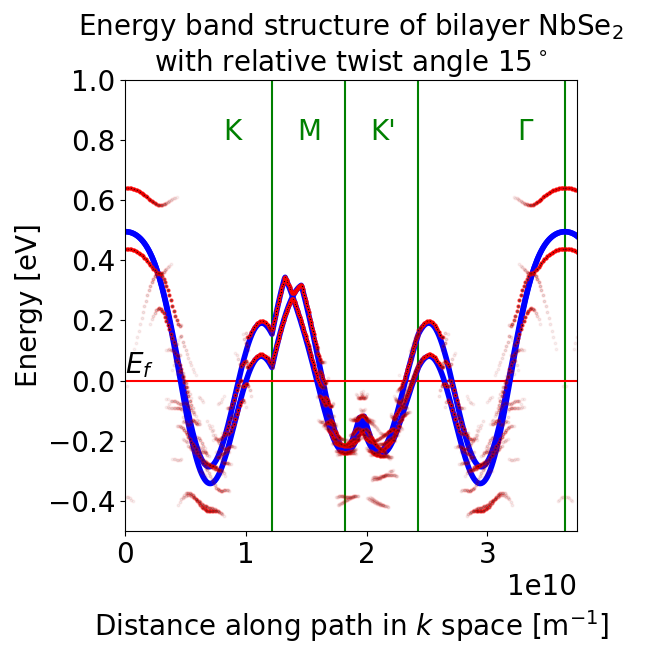
\includegraphics[width=0.95\textwidth]{0.1_coupling_15_deg.png}
    \caption{0.1 eV coupling}
    \label{bilayer_coupling_0.1}
  \end{subfigure}
  \vskip
  \baselineskip
  \begin{subfigure}[b]{0.475\textwidth}
    \centering
    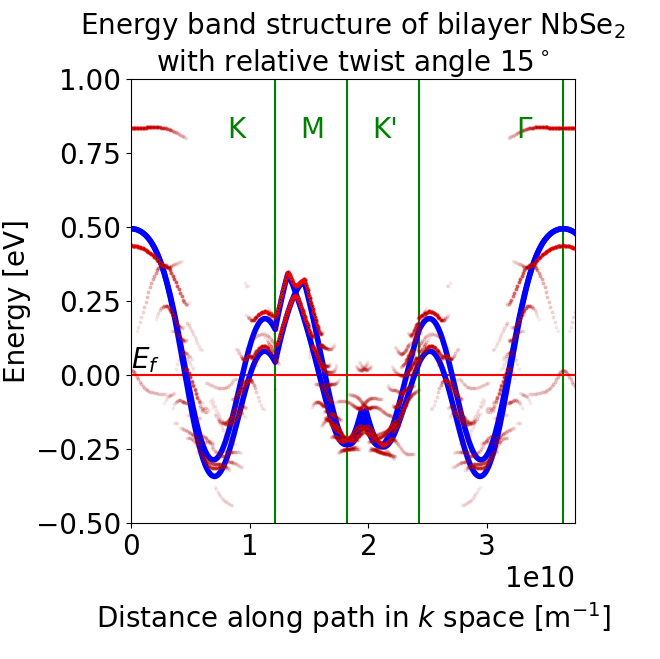
\includegraphics[width=0.95\textwidth]{0.2_coupling_15_deg.png}
    \caption{0.2 eV coupling}
    \label{bilayer_coupling_0.2}
  \end{subfigure}
  \hfill
  \begin{subfigure}[b]{0.475\textwidth}
    \centering
    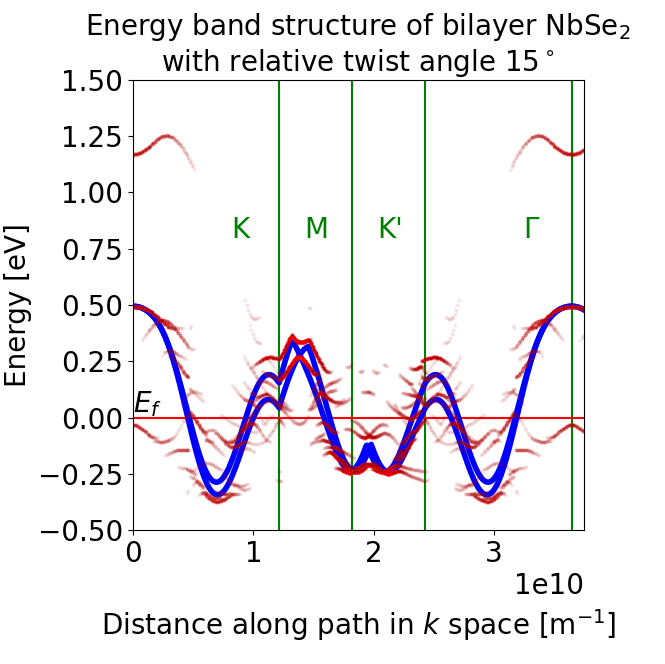
\includegraphics[width=0.95\textwidth]{0.4_coupling_15_deg.png}
    \caption{0.4 eV coupling}
    \label{bilayer_coupling_0.4}
  \end{subfigure}
  \caption{
    Altering the fixed interlayer coupling potential at a fixed twist angle of $15^\circ$. In experimentation we would expect to see coupling potentials \~ 0.1 eV \cite{}. The perturbation introduced by the coupling causes the electronic bands to seperate near degenerate points as in (\ref{perturbation_matrix, perturbation_energy})
  }
  \label{bilayer_bands_projected_coupling}
\end{figure*}

twist angle effect

\begin{figure*}[t]
\centering
  \begin{subfigure}[b]{0.475\textwidth}
    \centering
    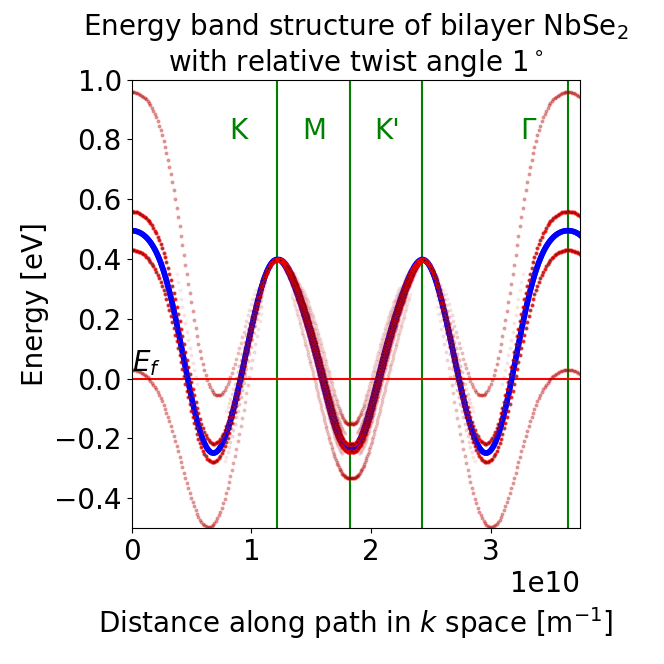
\includegraphics[width=0.95\textwidth]{1_deg_0.1_coupling.png}
    \caption{}
    \label{bilayer_rotation_1}
  \end{subfigure}
  \hfill
  \begin{subfigure}[b]{0.475\textwidth}
    \centering
    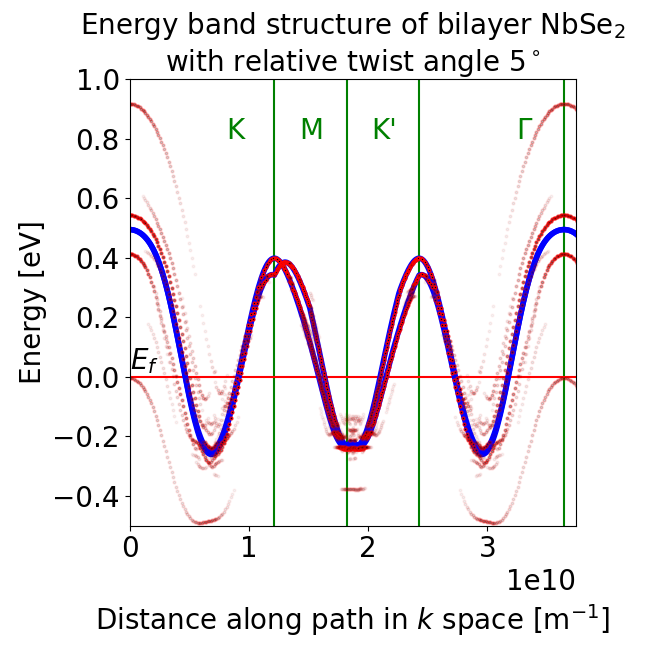
\includegraphics[width=0.95\textwidth]{5_deg_0.1_coupling.png}
    \caption{}
    \label{bilayer_rotation_5}
  \end{subfigure}
  \vskip
  \baselineskip
  \begin{subfigure}[b]{0.475\textwidth}
    \centering
    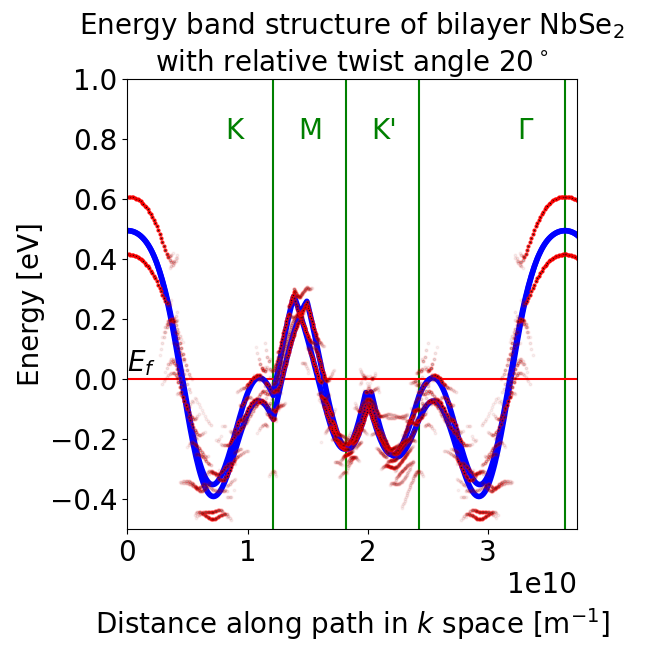
\includegraphics[width=0.95\textwidth]{20_deg_0.1_coupling.png}
    \caption{}
    \label{bilayer_rotation_20}
  \end{subfigure}
  \hfill
  \begin{subfigure}[b]{0.475\textwidth}
    \centering
    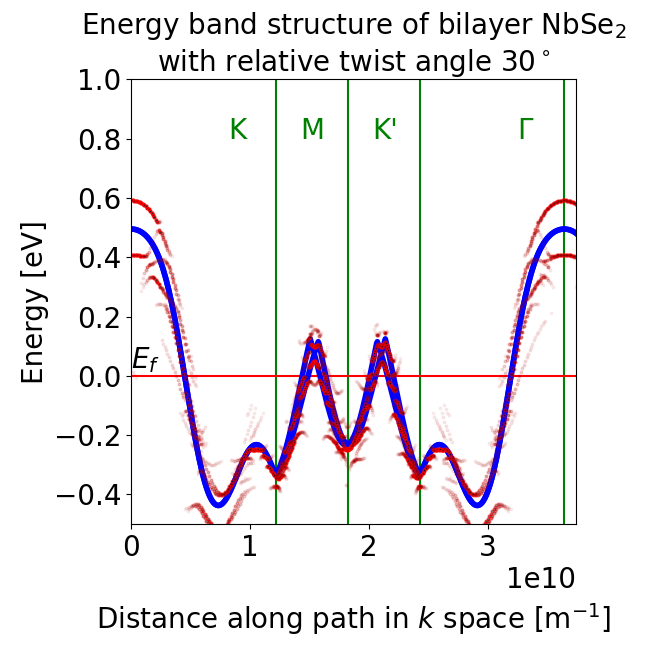
\includegraphics[width=0.95\textwidth]{30_deg_0.1_coupling.png}
    \caption{}
    \label{bilayer_rotation_30}
  \end{subfigure}
  \caption{
    Altering the relative interlayer twist angle at a fixed coupling potential of 0.1 eV. Some twist angles produce flat or nearly flat electronic bands associated with a high density of states.
  }
  \label{bilayer_bands_projected_rotation}
\end{figure*}

zoom into flat bands?

\begin{figure*}[t!]
\centering
  \begin{subfigure}[t]{0.45\textwidth}
    \centering
    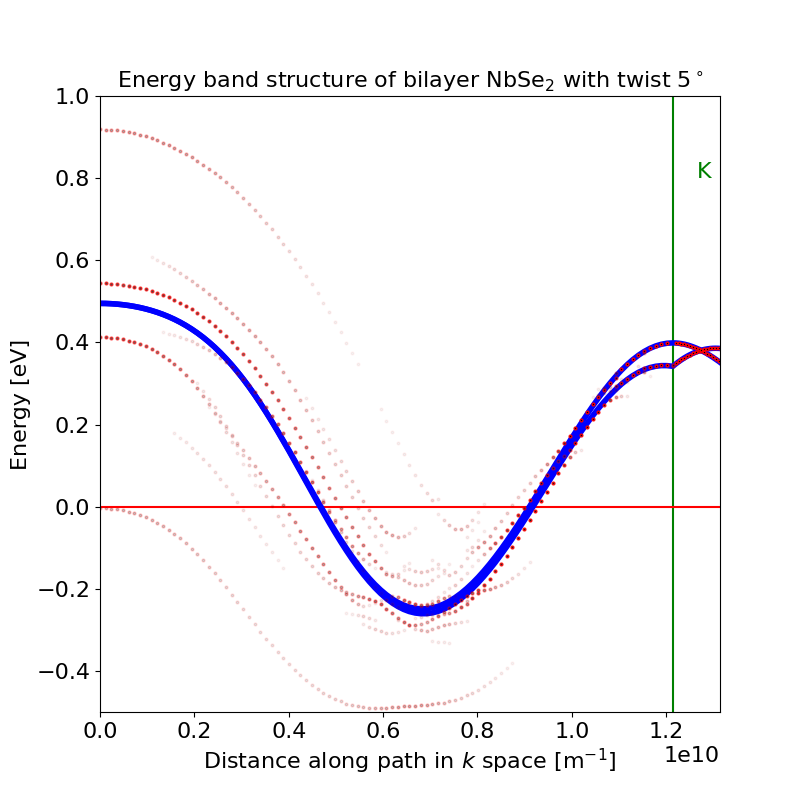
\includegraphics[width=0.95\textwidth]{bilayer_bands_5_projected_low_E_saddle.png}
    \caption{
    }
    \label{bilayer_bands_5_projected_low_E_saddle}
  \end{subfigure}
  \hfill
  \begin{subfigure}[t]{0.45\textwidth}
    \centering
    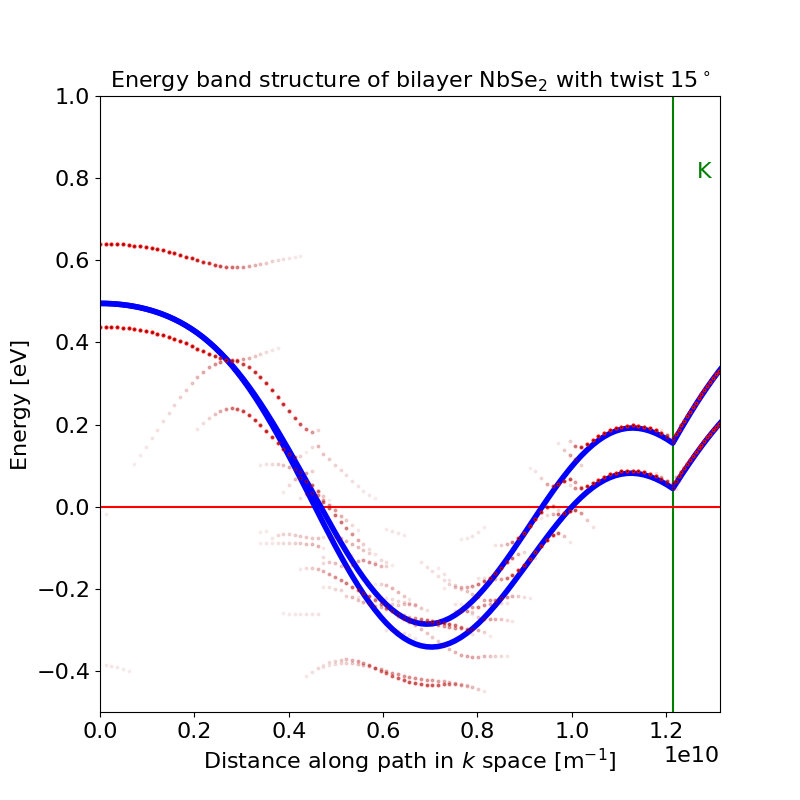
\includegraphics[width=0.95\textwidth]{bilayer_bands_15_projected_low_E_saddle.png}
    \caption{
    }
    \label{bilayer_bands_15_projected_low_E_saddle}
  \end{subfigure}
  \caption{}
  \label{bilayer_bands_projected_low_E_saddle}
\end{figure*}


\section*{Discussion}
discuss

approximations

coupling potential massively approximated as a const
probably the main approx

k 1,2,3,4 etc should couple to futher k (negligible but could go to second order)

limitations -> computation, sampling of k not actually quantised properly (doesnt matter really)

\section*{Conclusions}

conclude

\section*{Acknowledgements}
I would like to acknowledge the contributions of my project partner Sanjana Reddy and my project supervisor Dr Marcin Mucha-Kruczynski.

%%%References
\bibliographystyle{ieeetr}
%bibliographystyle{bathx}
\bibliography{refs}

\clearpage

\onecolumn

\section*{Appendix}

\subsection*{Inter-layer tunneling Hamiltonian derivation}

\subsection*{Implementation of algorithm}
  Modelling, data analysis and plotting were performed in Python using the NumPy and matplotlib libraries. All computations were performed on 64-bit processors either running Linux Mint 20.3 , Ubuntu Linux 20.04.4 LTS on WSL or Windows 10 home edition.

  \textbf{Note: }

  Code example
\begin{lstlisting}
//write recorded data to a CSV file
void DLASystem::writeDataCSV(){
  auto csv = new CSVWrite("./data.csv");

  csv->WriteVector(dataSet);
  csv->CSVClose();

  //clearDataSet();

  recording = false; //should be false anyways
}
\end{lstlisting}

\end{document}
